\section*{Week 5: Acquisitions / Financial Investments}

\subsection*{Acquisitions and goodwill}


Steps for \textit{allocating the purchase price} :
\begin{enumerate}[noitemsep,topsep=0pt]
	\item Fair value of tangigle assets and liabilities.
	\item \textit{Identifiable} intangile assets: customer relationships, trade names, patents, etc. Subject to amortization with zero salvage value.
	\item Goodwill.  An intangible assets that is not separately identifiable: Everything else (the plug).
\end{enumerate}

\subsection*{Investments}

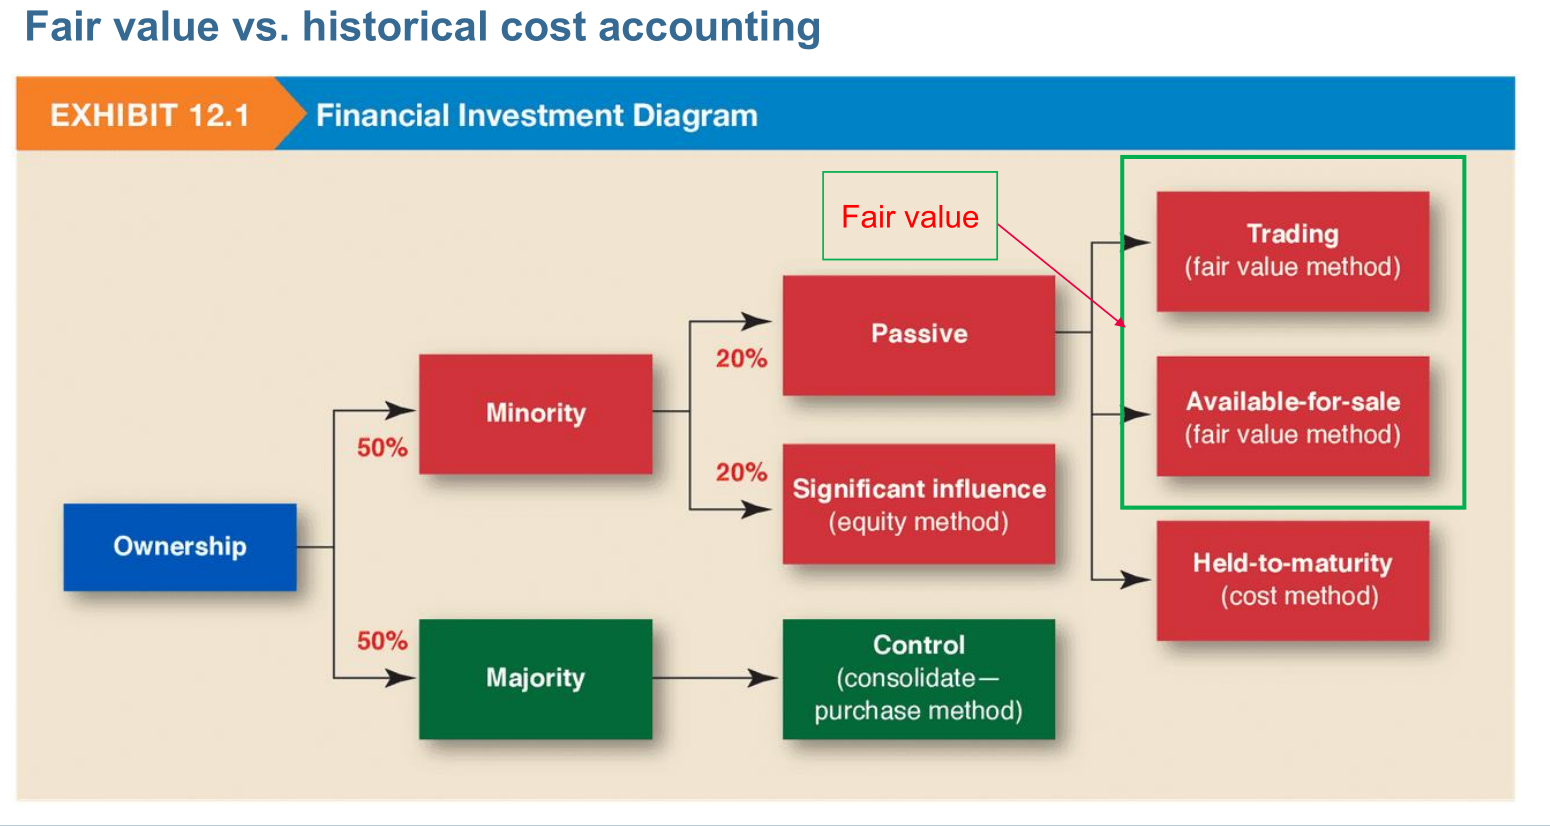
\includegraphics[width=7cm]{assets/fair_value_vs_historical_acct}

\subsection*{Equity Method}

\begin{itemize}[noitemsep,topsep=0pt]
	\item Initially record the investment at acquisition cost.
	\item Adjust the book value of the investment by the investor’s share of dividends and
	earnings or losses.
	\item Record investor’s share of investee’s profit on the investor’s income statements.
	\item Dividends received reduce investment; they do not give rise to dividend income.
\end{itemize}




\textbf{Accounting treatment un unrealized gains/losses accross categories for passive investments}
\\
HTM: Hold to maturity \\
AFS: Available for sale \\
TRD: Trading \\
\begin{center}
	\begin{tabular}{ |c|c|c| } 
		\hline
			  & B/S Effect & I/S Effect \\ 
		\hline
		HTM & no &  \\ 
		AFS & yes & no \\ 
		TRD & yes & yes \\ 
		\hline
	\end{tabular}
\end{center}

Changes in market value affect the balance sheet for AFS and TRD securities. Changes in market value affect income statement only for TRD securiteis.